%%!TEX root = ./UserManual.tex
\chapter{Simulator}
\label{chap:simulator}


%%%%%%%%%%%%%%%%%%%%%%%%%%%%%%%%%%%%%%%%%%%%%%%%%%%%%%%%%%%%%%%%
% Workspace
%%%%%%%%%%%%%%%%%%%%%%%%%%%%%%%%%%%%%%%%%%%%%%%%%%%%%%%%%%%%%%%%
\section{Workspace}

By default, \texttt{Stride} is installed in \texttt{./target/installed/} inside de project directory. This can be modified by setting the \texttt{CMAKE\_INSTALL\_PREFIX} on the CMake command line (see the \texttt{INSTALL.txt} file in the prject root directory) or by using the CMakeLocalConfig.txt file (example file can be found  in \texttt{./src/main/resources/make}).

Compilation and installation of the software creates the following files and directories:
\begin{compactitem}
%
	\item Binaries in directory \texttt{<install\_dir>/bin}
      		\begin{compactitem}
        			\item $stride$: executable.
        			\item $gtester$: regression tests for the sequential code.
               	 \item $gengeopop$: generates the population and geographical grid.
        			\item $wrapper\_sim.py$: Python simulation wrapper
        	\end{compactitem}
%
    \item Configuration files (xml and json) in directory \texttt{<install\_dir>/config}
      	\begin{compactitem}
			\item $run\_default.xml$: default configuration file for Stride to perform a Nassau simulation.
        		\item $run\_generate\_default.xml$: default configuration file for Stride to first generate a population and geographical grid, then perform a Nassau Simulation and at the same time create epi-output.
       		\item $run\_import\_default.xml$: default configuration file for Stride to first import a population and geographical grid and then perform a Nassau Simulation.
        		\item $run\_miami\_weekend.xml$: configuration file for Stride to perform Miami simulations with uniform social contact rates in the community clusters.
			\item $wrapper\_miami.json$: default configuration file for the wrapper\_sim binary to perform Miami simulations with different attack rates.
        		\item \ldots
        \end{compactitem}
%        
    \item Data files (csv) in directory \texttt{<project\_dir>/data}
      	\begin{compactitem}
        		\item $belgium\_commuting$: Belgian commuting data for the active populations. The fraction of residents from ``city\_depart'' that are employed in ``city\_arrival''. Details are provided for all cities and for 13 major cities.
			\item $belgium\_population$: Relative Belgian population per city. Details are provided for all cities and for 13 major cities.
        	\item $flanders\_cities$: Cities and municipalities in Flanders with coordinates and population figures based on samples. These relative population figures are used for assigning residencies and domiciles based on a discrete probability distribution.
        	\item $flanders\_commuting$: Relative commuting information between cities and communities. Since this data is relative, the total number of commuters is a derived parameter, based on the fraction of the total population that is commuting.
			\item $contact\_matrix\_average$: Social contact rates, given the cluster type. Community clusters have average (week/weekend) rates.
			\item $contact\_matrix\_week$: Social contact rates, given the cluster type. Community clusters have week rates.
			\item $contact\_matrix\_week$: Social contact rates, given the cluster type. Primary Community cluster has weekend rates, Secondary Community has week rates.
			\item $disease\_xxx$: Disease characteristics (incubation and infectious period) for xxx.
			\item $holidays\_xxx$: Holiday characteristics for xxx.
			\item $ref\_2011$: Reference data from EUROSTAT on the Belgian population of 2011. Population ages and household sizes.
			\item $ref\_fl2010\_xxx$: Reference data on social contacts for Belgium, 2011.
        \end{compactitem}
%
    \item Documentation files in directory \texttt{./target/installed/doc}
      	\begin{compactitem}
        			\item Reference manual
        			\item User manual
        \end{compactitem}
%
\end{compactitem}

The install directory is also the workspace for \texttt{Stride}. The \texttt{Stride} executable allows you to use a different output directory for each new calculation (see the next section).

%%%%%%%%%%%%%%%%%%%%%%%%%%%%%%%%%%%%%%%%%%%%%%%%%%%%%%%%%%%%%%%%
% Run
%%%%%%%%%%%%%%%%%%%%%%%%%%%%%%%%%%%%%%%%%%%%%%%%%%%%%%%%%%%%%%%%
\newpage
\section{Running the simulator}

From the workspace directory, the simulator can be started  using the command \mbox{``\texttt{./bin/stride}''}. Arguments can be passed to the simulator on the command line:
\begin{verbatim}

USAGE: 
 
   bin/stride  [-e <clean|dump|sim|genpop>] [-c <CONFIGURATION>] [-o
               <<NAME>=<VALUE>>] ...  [-i] [--stan <COUNT>] [--]
               [--version] [-h]
               
Where: 
 
   -e <clean|dump|sim|genpop>,  --exec <clean|dump|sim|genpop>
     Execute the corresponding function:  
 
         clean:  cleans configuration and writes it to a new file.  
 
         dump:   takes built-in configuration writes it to a file.  
 
         sim:    runs the simulator and is the default.  
 
         genpop: generates geo-based population to file (no sim)
 
     Defaults to --exec sim.
 
   -c <CONFIGURATION>,  --config <CONFIGURATION>
     Specifies the run configuration parameters. The format may be either
     -c file=<file> or -c name=<name>. The first is mostly used and may be
     shortened to -c <file>. The second refers to built-in configurations
     specified by their name.
 
     Defaults to -c file=run_default.xml
 
   -o <<NAME>=<VALUE>>,  --override <<NAME>=<VALUE>>  (accepted multiple
      times)
     Override configuration file parameters with values provided here.
 
   -i,  --installed
     File are read from the appropriate (config, data) directories of the
     stride install directory. If false, files are read and written to the
     local directory. 
 
     Defaults to true.
 
   --stan <COUNT>
     Stochastic Analysis (stan) will run <COUNT> simulations, each with a
     different seed for the random engine. Only applies in case of -e sim.
 
   --,  --ignore_rest
     Ignores the rest of the labeled arguments following this flag.
 
   --version
     Displays version information and exits.
 
   -h,  --help
     Displays usage information and exits.

\end{verbatim}

For example if you run with the default configuration file, but you
want to change the logging level,
(choices are: \texttt{trace}, \texttt{debug}, \texttt{info}, \texttt{warn},
\texttt{error}, \texttt{critical}, \texttt{off})) execute:\\
\verb!         stride --override stride_log_level=error!


%%%%%%%%%%%%%%%%%%%%%%%%%%%%%%%%%%%%%%%%%%%%%%%%%%%%%%%%%%%%%%%%
% Wrapper
%%%%%%%%%%%%%%%%%%%%%%%%%%%%%%%%%%%%%%%%%%%%%%%%%%%%%%%%%%%%%%%%
\section{Python Wrapper}
A Python wrapper is provided to perform multiple runs with the C++ executable.
The wrapper is designed to be used with .json configuration files and examples are provided with the source code.
For example: \\ \\
\centerline{\texttt{./bin/wrapper\_sim --config ./config/wrapper\_default.json}} \\ \\
will start the simulator with each configuration in the file.
It is important to note the input notation: values given inside brackets can be extended (e.g., ``rng\_seeds''=[1,2,3]) but single values can only be replaced by one other value (e.g., ``days'': 100).


%%%%%%%%%%%%%%%%%%%%%%%%%%%%%%%%%%%%%%%%%%%%%%%%%%%%%%%%%%%%%%%%
% Visualizer
%%%%%%%%%%%%%%%%%%%%%%%%%%%%%%%%%%%%%%%%%%%%%%%%%%%%%%%%%%%%%%%%
\section{Running the visualization}	

From the workspace directory, the visualization can be started  using the command \mbox{``\texttt{./bin/visualization/strideVisualization}''}. One argument has to be passed to the visualization on the command line, which is the epi-output file that will be read and represented. For example: \\ \\
\centerline{\texttt{./bin/visualization/strideVisualization \textless EPI-OUTPUT\textgreater}} \\ \\
In the GUI you can select an area to get the epi-output of that area, selections can be made with the right mouse button.

\begin{center}
	\begin{figure}[hbtp!]
		\makebox[\textwidth][c]{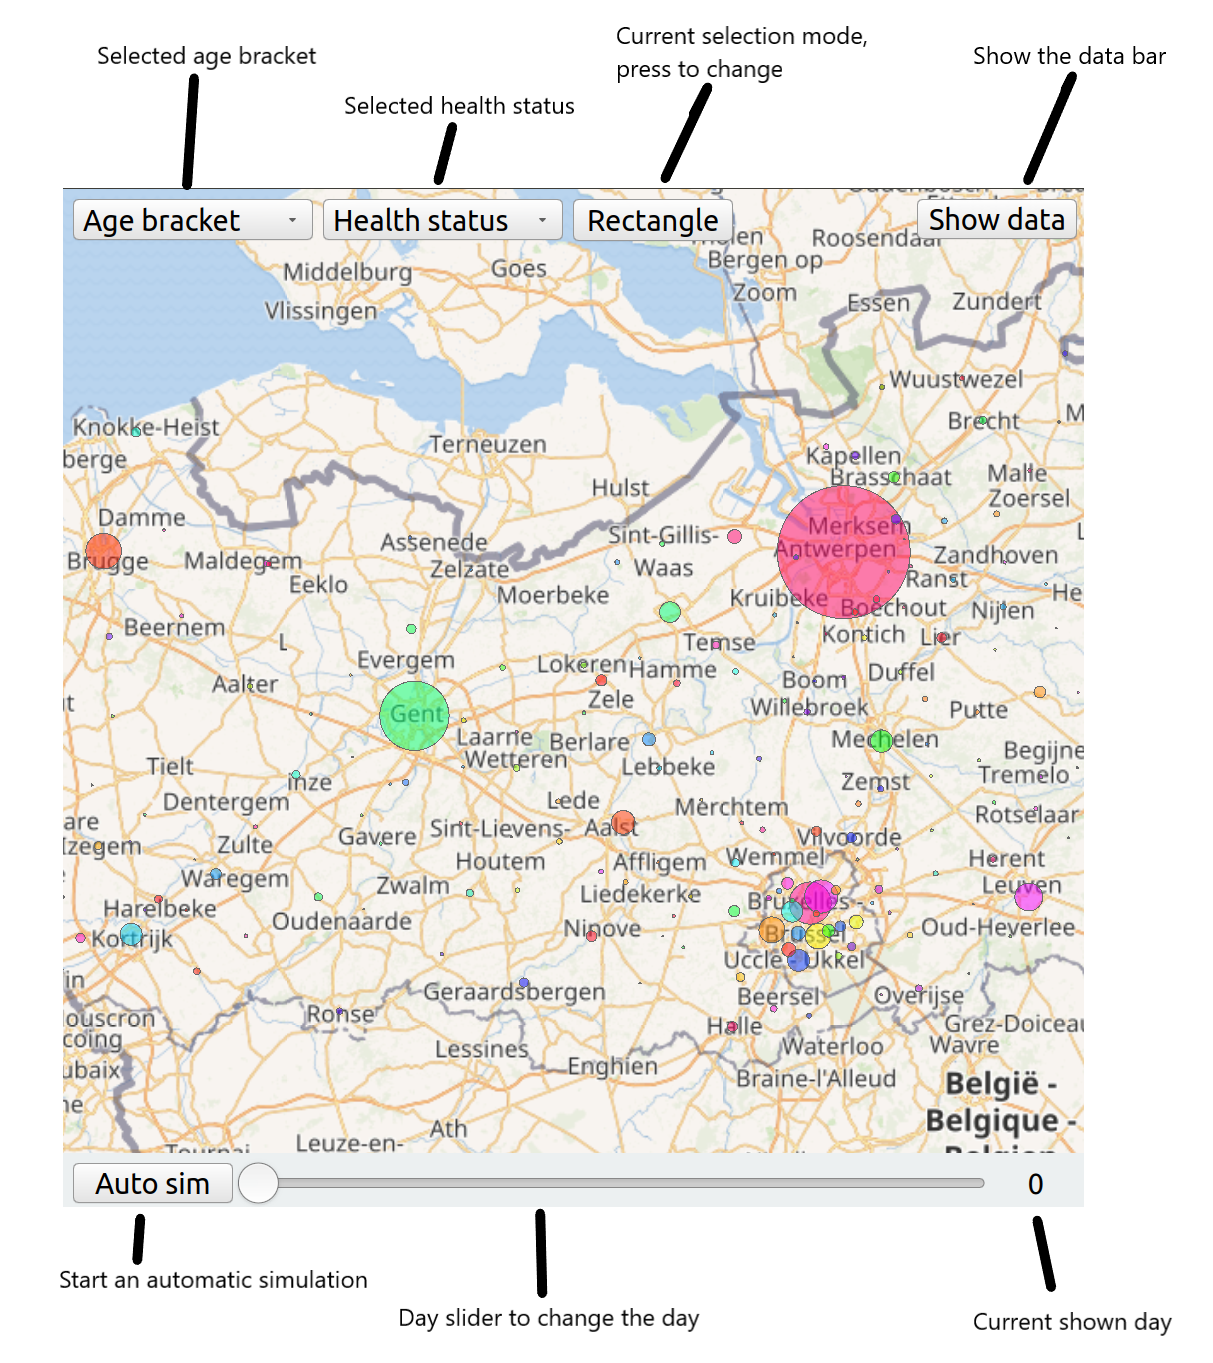
\includegraphics[width=1.2\textwidth]{GUI1.png}}%
		\caption{GUI part 1} \label{gui1}
	\end{figure}
\end{center}

\begin{center}
	\begin{figure}[hbtp!]
		\makebox[\textwidth][c]{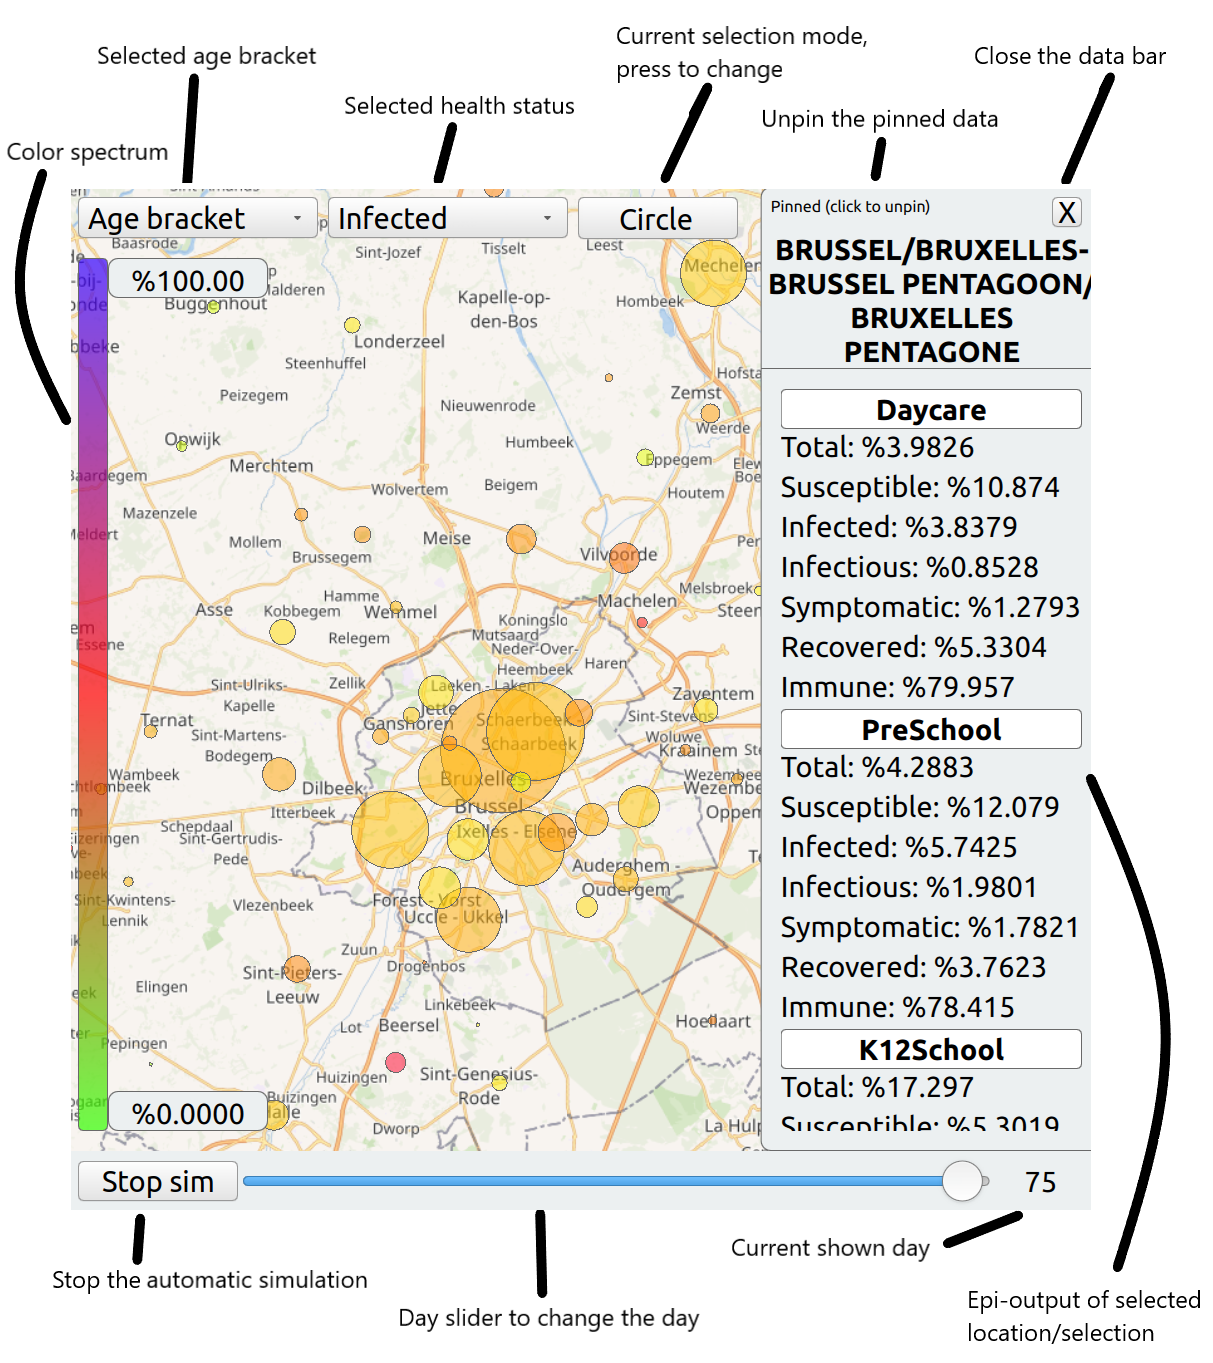
\includegraphics[width=1.2\textwidth]{GUI2.png}}%
		\caption{GUI part 2} \label{gui2}
	\end{figure}
\end{center}


